\section{Monitoring and Calibration Suites}

\subsection{Calibration Framework}

A calibration framework was developed to implement visualization software tools needed for all detector
systems. Standard views were developed using the JAVA Swing application to visualize detector components and to provide callback
mechanisms necessary to display detector-component specific information.  These software tools provide
functionality for data fitting, plotting and displaying using a graphical user interface environment.

The calibration framework makes use of the other CLAS12 libraries
(the geometry and plotting packages, as well as database utilities) and provides a uniform Graphical User
Interface (GUI) for all calibration applications. The framework provides a data processing interface
and a calibration constant database interface used
for on- and off-line data analysis.

A common data streaming interface is implemented with software level abstraction that allows calibration and monitoring
code to run on variety of supported data formats used in CLAS12.

%%%%%%%%%%%%%%%%%%%%%%%%%%%%%%%%%%%%%%%%%%%%%%%%%%%%%%%%%%
\begin{figure*}
\centering
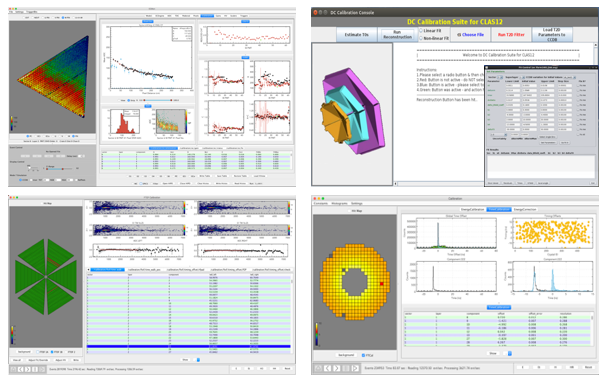
\includegraphics[width=0.8\textwidth]{pics/suites.png}
\caption{Representative subsystem calibration GUIs for ECAL~\cite{ecal-nim} (upper left),
DC~\cite{dc-nim} (upper right), FTOF~\cite{ftof-nim} (lower left),  and FT~\cite{ft-nim} (lower right).}
\label{suites}
\end{figure*}
%%%%%%%%%%%%%%%%%%%%%%%%%%%%%%%%%%%%%%%%%%%%%%%%%%%%%%%%%%%

\subsection{Calibration Suites}

The software programs used for the CLAS12 detector subsystem monitoring and energy and time calibrations are
Java-based suites that employ the framework discussed in Section~\ref{common-tools}.
The software tools provided by the framework facilitate the development of
detector-specific suites. Fig.~\ref{suites} shows representative views of CLAS12 subsystem calibration suites.

The calibration applications take as input raw or reconstructed data files
(from either beam data or Monte Carlo simulations) in
either EVIO or HIPO data formats.  They display the various quantities and histograms relevant to the
extraction of the calibration constants.  Each calibration suite performs fits to determine the detector subsystem
the calibration constants.  The calibration analysis parameters are saved into ASCII files
with the same structure as the tables defined in CCDB.

\subsection{Timelines}
~~

\section{CLAS12 Event Display}
The CLAS Event Display (ced) is a diagnostic graphical application for displaying CLAS events.
The primary element of ced is the view. A view is a graphical representation of CLAS in its
entirety or a subset of detector packages.
ced contains multiple views of CLAS, some geometrically faithful and some not.
It has both 2-dimensional and 3-dimensional views. Some views are purely informational, typically in the form of tables.
An illustration of views in ced is shown in Fig.~\ref{fig:dcTracks}.

